\documentclass[12pt]{amsart}
\usepackage[fullpage]{geometry}
\usepackage{fullpage}
\usepackage{pbox}
\usepackage{graphicx}
\usepackage{booktabs} % Top and bottom rules for table
\usepackage{amsfonts, amsmath, amsthm, amssymb}
\usepackage{longtable,array,color,xcolor}
\usepackage[colorlinks = true,
            urlcolor  = blue]{hyperref}
\usepackage{verbatim}
\usepackage{enumerate}
\newcommand\narrowstyle{\SetTracking{encoding=*}{-50}\lsstyle}
\newcommand{\RR}{\mathbb{R}}

\setlength{\parindent}{0pt}

\begin{document}

\title{Math 320: Homework 7}
Due: November 18, 2016
\maketitle

Please read through chapters 14, 15.1-15.3, and 17 in the textbook.
Answer the following questions. Please submit all code
and output with brief descriptions of what you are doing.

\vspace{5mm}

\begin{enumerate}

\item Problem 14.5

The data is below:
\[
\begin{array}{|c|cccccccccc|} \hline
x & 0 & 2 & 4 & 6 & 9 & 11 & 12 & 15 & 17 & 19 \\ \hline
y & 5 & 6 & 7 & 6 & 9 & 8 & 8 & 10 & 12 & 12 \\ \hline
\end{array}
\]

The following code is used to compute the regression line,
the standard error of the estimate, and the correlation coefficient
-- all for the regression line of $y$ versus $x$.

\begin{verbatim}
X = [0 2 4 6 9 11 12 15 17 19;
    5 6 7 6 9 8 8 10 12 12]

%x-regression

A = [ones(10,1) X(1,:)']
b = [X(2,:)']
beta = A'*A \ A'*b

%Plotting the data & Regression line
plot(X(1,:),X(2,:),'.')
axis([-2 20 3 15])
hold on 
plot([-2,20],[beta(1) + beta(2)*-2,
    beta(1) + beta(2)*20]);

%Std Error & Correlation computation
sr = sum((beta(1) + beta(2)*X(1,:) - X(2,:)).^2);
syx = sqrt(sr/(10-2));
st = sum((X(2,:) - mean(X(2,:))).^2);
r = ((st - sr)/st)^(1/2)
\end{verbatim}

\vspace{5mm}

\begin{tabular}{lr}
Regression line & $Y = 4.8881 + .3591 X$ \\
Standard error of the estimate & .8511 \\
Correlation coefficient & .9449 \\
\end{tabular}

\pagebreak

The following code is used to compute the regression line,
the standard error of the estimate, and the correlation coefficient
-- all for the regression line of $x$ versus $y$.



\begin{verbatim}
%y-regression

A = [ones(10,1) X(2,:)']
b = [X(1,:)']
beta = A'*A \ A'*b

plot(X(1,:),X(2,:),'.')
axis([-2 20 3 15])
hold on 
plot([beta(1) + beta(2)*3,
    beta(1) + beta(2)*15],[3,15])

sr = sum((beta(1) + beta(2)*X(2,:) - X(1,:)).^2);
sxy = sqrt(sr/(10-2))
st = sum((X(1,:) - mean(X(1,:))).^2);
r = ((st - sr)/st)^(1/2)
\end{verbatim}

\vspace{5mm}


\begin{tabular}{lr}
Regression line & $X = -11.1349 + 2.4861Y$ \\
Standard error of the estimate & 2.2393 \\
Correlation coefficient & .9449 \\
\end{tabular}

\vspace{5mm}

The plot at left is for the regression of $y$ versus $x$; the plot
at right is the regression of $x$ versus $y$.

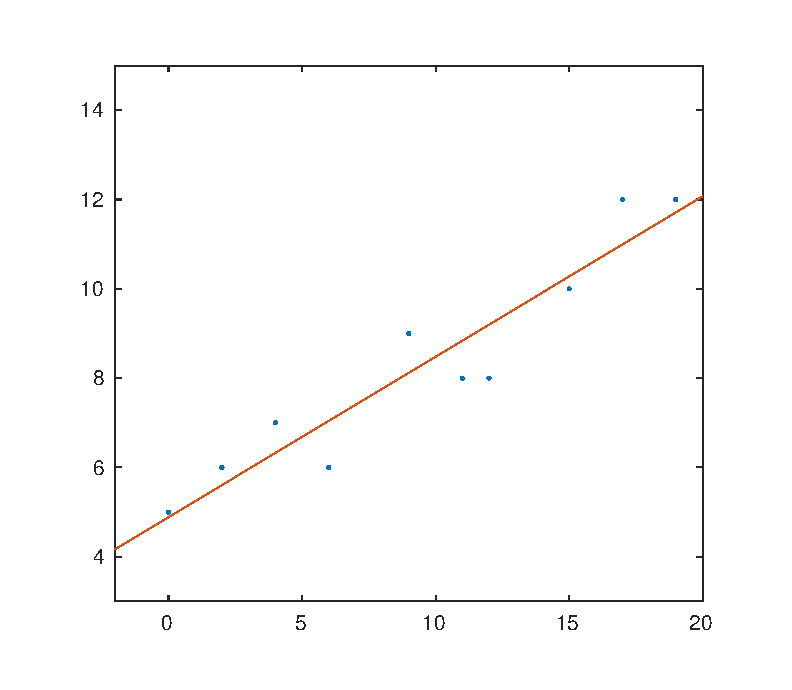
\includegraphics[width=.45\textwidth, height=7cm]{p1xline.eps}
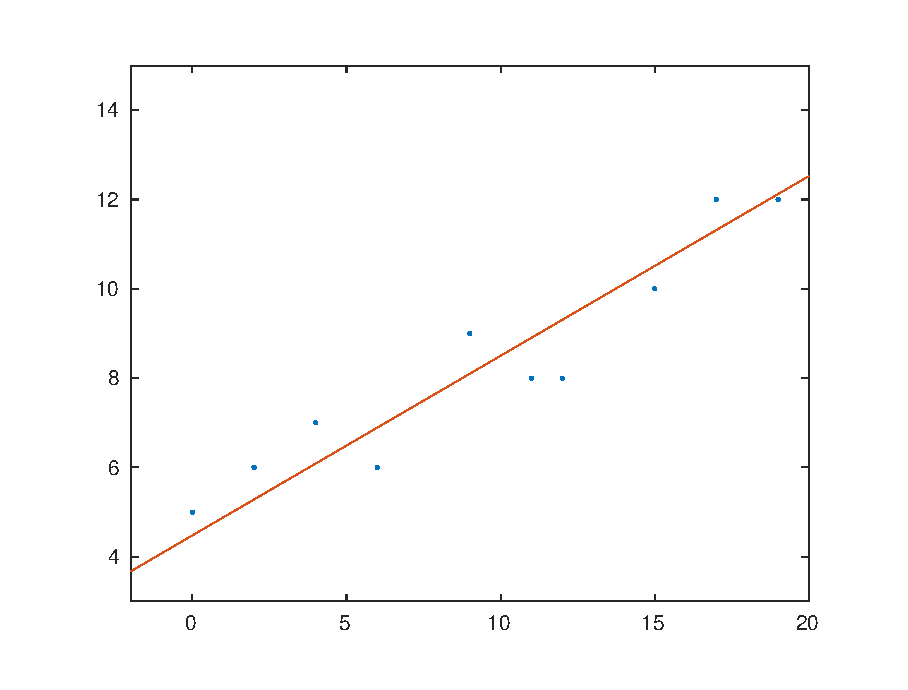
\includegraphics[width=.45\textwidth, height= 7cm]{p1yline.eps}


\vfill
\pagebreak









\item Problem 14.34

\vspace{5mm}

We carry out the Monte Carlo simulation using the
following MATLAB code:

\vspace{1cm}

\begin{verbatim}
Q = @(nm,B,H,S) (1/nm)*((B*H)^(5/3)/(B+2*H)^(2/3))*sqrt(S)
% Note B = 20, H = 0.3
% nm in range (0.027,0.033)
% S  in range (0.00027,0.00033)

in = rand(2,10000);
in(1,:) = .027 + .006*in(1,:);
in(2,:) = .00027 + .00006*in(2,:);
Qdata = zeros(1,10000);
for i=1:10000
    Qdata(i) = Q(in(1,i),20,0.3,in(2,i));
end
histogram(Qdata, 50)
\end{verbatim}

\vspace{1cm}

The following histograms were obtained using
two trials:

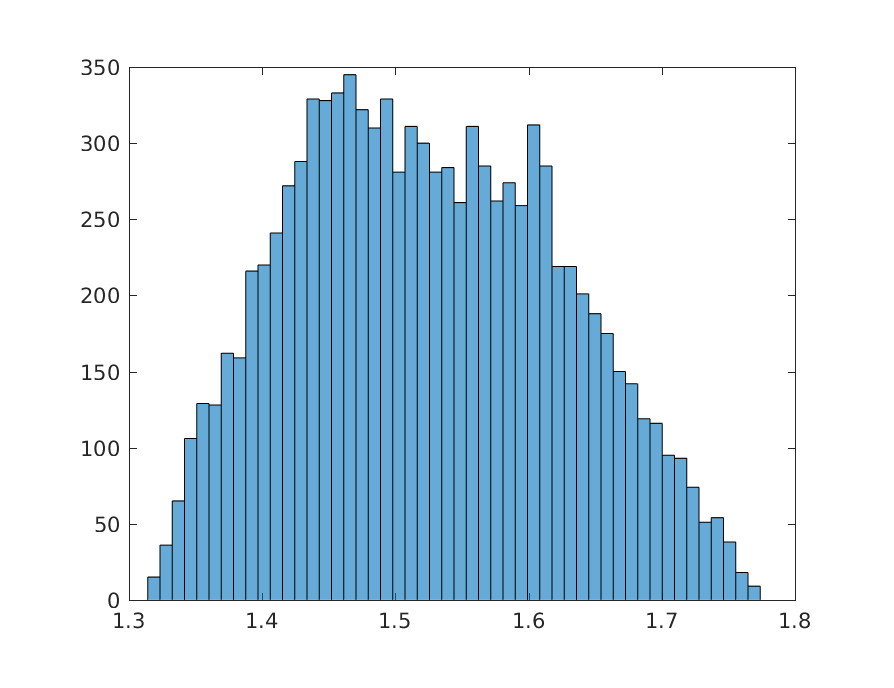
\includegraphics[width=.5\textwidth]{p2histA.eps}
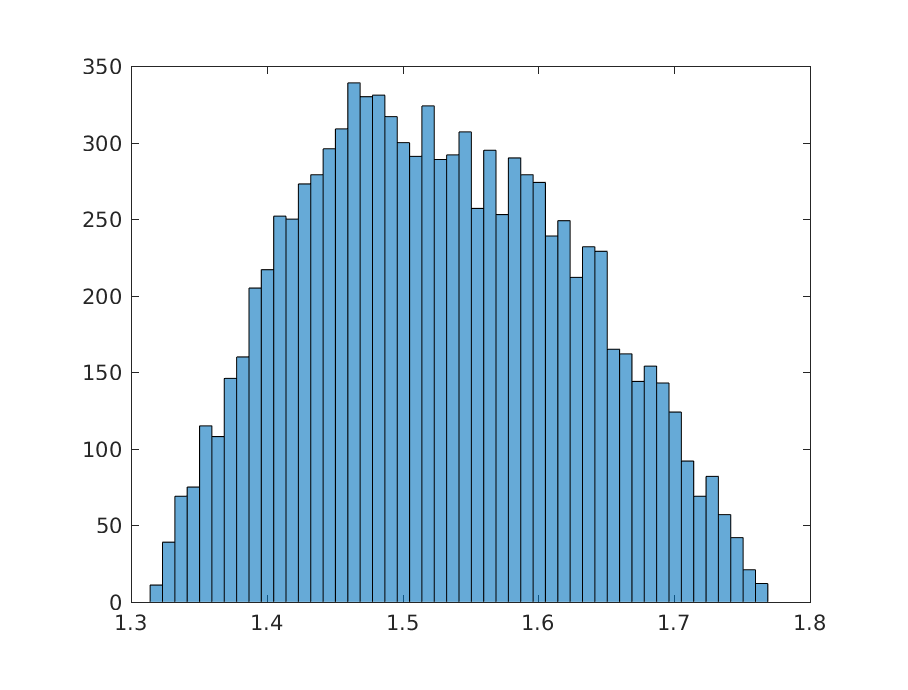
\includegraphics[width=.5\textwidth]{p2histB.eps}






\vfill
\pagebreak

\item Problem 15.12


\vspace{5mm}

\[
\begin{array}{|c|ccccc|} \hline
x & 1 & 2 & 3 & 4 & 5 \\ \hline
y & 2.2 & 2.8 & 3.6 & 4.5 & 5.5 \\ \hline
\end{array}
\]

The MATLAB code we use to analyze this data and
fit it to the model
\[ y = a + bx + \dfrac{c}{x}\]
is below:

\begin{verbatim}
X = [1 2 3 4 5]';
Y = [2.2 2.8 3.6 4.5 5.5]';

A = [ones(5,1) X X.^(-1)];
b = A'*A \ A'*Y

f = @(x) b(1) + b(2)*x + b(3)*(1/x);
X2 = .8:0.05:5.2; Y2 = arrayfun(f,X2);
plot(X,Y,'.',X2,Y2)
\end{verbatim}

The regression yields $Y = 0.3745 + 0.9864 X + \dfrac{ 0.8456}{X}$, which 
is depicted below.

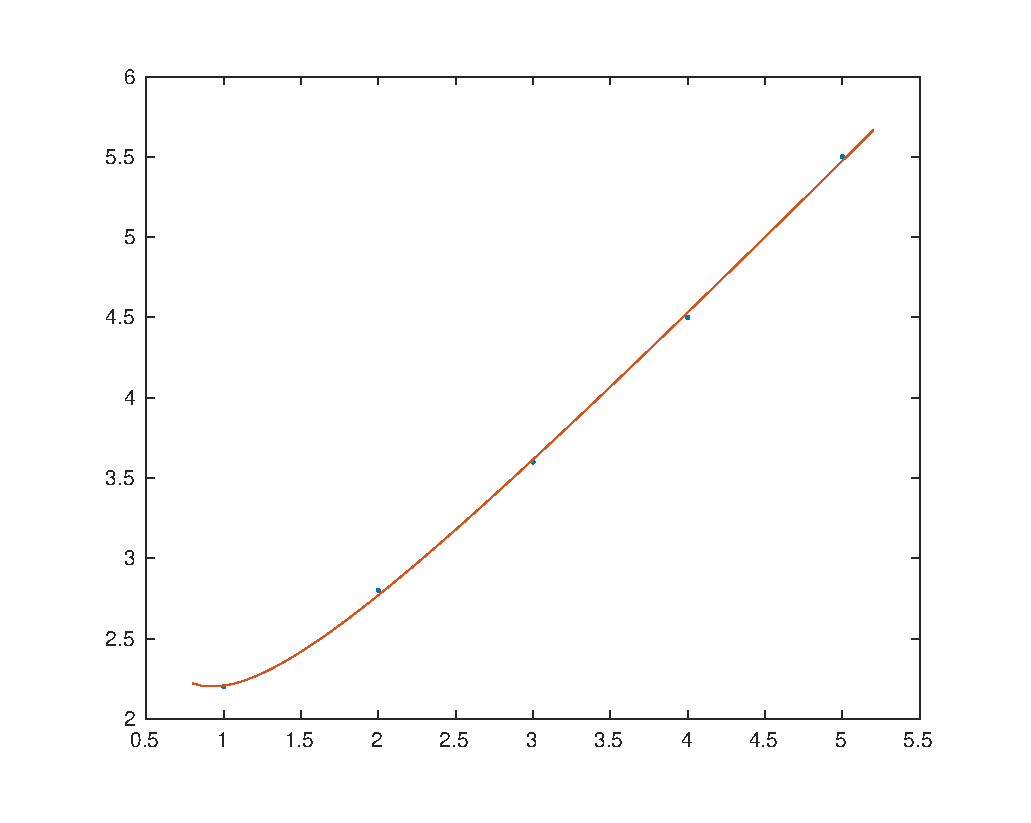
\includegraphics[width=.8\textwidth]{p3fit.eps}
\vfill
\pagebreak

\item Let $z = f(x,y)$ be a function of two variables. \\
 Suppose
we have the following $6$ points:
\[
\begin{array}{|c|cccccc|} \hline
x & 1 & 1 & 2 & 2 & 3 & 3 \\
y & 2 & 3 & 1 & 3 & 1 & 2 \\
z & 3 & 2 & 3 & 1 & 2 & 1 \\ \hline
\end{array}
\]
Find a degree-5 homogeneous polynomial in $x$ and $y$
that includes these six points. Plot the corresponding
surface in MATLAB.

\vspace{5mm}

We can treat this like a standard linear algebra problem--
a homogeneous degree-5 polynomial has six terms:
\[F(X,Y) = \beta_5 X^5 + \beta_4 X^4Y + \beta_3 X^3Y^2 + \beta_2 X^2Y^3 + \beta_1 XY^4 + \beta_0 Y^5.\] 

In matrix form:
\[ \left(
\begin{array}{cccccc}
| & | & | & | & | & | \\
 X^5  & X^4Y &  X^3Y^2  & X^2Y^3 & XY^4 &  Y^5 \\
| & | & | & | & | & | \\
\end{array}\right)
\left( \begin{array}{c}
| \\ \beta \\ | \end{array}
\right) =
\left( \begin{array}{c}
| \\ Z \\ | \end{array}
\right)
\]
Row $i$ of the $XY$ matrix corresponds to data point $(x_i,y_i)$
and coordinate $i$ of the $Z$ vector gives the value of $z_i$.

After evaluating everything, the equation is:
\[\left(
\begin{array}{cccccc}
     1  &   2 &    4 &    8 &   16 &   32 \\
     1  &   3 &    9 &   27 &   81 &  243 \\
    32  &  16 &    8 &    4 &    2 &    1 \\
    32  &  48 &   72 &  108 &  162 &  243 \\
   243  &  81 &   27 &    9 &    3 &    1 \\
   243  & 162 &  108 &   72 &   48 &   32 \\
\end{array}\right)
\left(\begin{array}{c} \beta_5 \\ \beta_4 \\ \beta_3 \\ \beta_2 \\ \beta_1 \\ \beta_0 \end{array} \right) = \left(
\begin{array}{c} 3 \\ 2 \\ 3 \\ 1 \\ 2 \\ 1 \end{array}
\right).\]

The MATLAB code to reach this equation and solve it, as
well as to plot the corresponding surface is below:

\begin{verbatim}
X = [1 1 2 2 3 3]';
Y = [2 3 1 3 1 2]';
Z = [3 2 3 1 2 1]';

A = [X.^5 X.^4.*Y X.^3.*Y.^2 X.^2.*Y.^3 X.*Y.^4 Y.^5];
beta = A \ Z

func = @(x,y) ([x.^5 x.^4.*y x.^3.*y.^2 x.^2.*y.^3 x.*y.^4 y.^5]*beta)(1)

fsurf(func,[0,3.5])
hold on
plot3(X,Y,Z,'b*')

\end{verbatim}

\includegraphics{p4.eps}

The blue stars signify the data points that we were trying to fit.

\end{enumerate}



\end{document}
